\documentclass{acm_proc_article-sp}

\usepackage[utf8]{inputenc}
\usepackage[T1]{fontenc}

\usepackage[activate=compatibility]{microtype}

% autoref command
\usepackage[pdftex,urlcolor=black,colorlinks=true,linkcolor=black,citecolor=black,draft]{hyperref}
\def\sectionautorefname{Section}
\def\subsectionautorefname{Subsection}
\def\subfloatautorefname{Subfigure}

\usepackage[lofdepth,lotdepth]{subfig}

\usepackage{enumitem}

\usepackage{mathtools}

% give emph a normal fontsize
\let\oldemph\emph
\renewcommand{\emph}[1]{\oldemph{\fontsize{9}{9}\selectfont #1}}

% more readable footnote layout
\renewcommand{\footnotesize}{\fontsize{8pt}{10pt}}
\setlength{\footnotesep}{.5cm}

% todo macro
\usepackage{color}
\newcommand{\todo}[1]{\noindent\textcolor{red}{{\bf \{TODO}: #1{\bf \}}}}

% listings and Verbatim environment
\usepackage{fancyvrb}
\usepackage{relsize}
\usepackage{listings}
\usepackage{verbatim}
\newcommand{\defaultlistingsize}{\fontsize{8pt}{9.5pt}}
\newcommand{\inlinelistingsize}{\fontsize{8pt}{11pt}}
\newcommand{\smalllistingsize}{\fontsize{7.5pt}{9.5pt}}
\newcommand{\listingsize}{\defaultlistingsize}
\RecustomVerbatimCommand{\Verb}{Verb}{fontsize=\inlinelistingsize}
\RecustomVerbatimEnvironment{Verbatim}{Verbatim}{fontsize=\defaultlistingsize}
\lstset{frame=lines,captionpos=b,numberbychapter=false,escapechar=§,
        aboveskip=0.5em,belowskip=0em,abovecaptionskip=0em,belowcaptionskip=0em,
framexbottommargin=-1em,
        basicstyle=\ttfamily\listingsize\selectfont}

% use Courier from this point onward
\let\oldttdefault\ttdefault
\renewcommand{\ttdefault}{pcr}
\let\oldurl\url
\renewcommand{\url}[1]{\inlinelistingsize\oldurl{#1}}

% linewrap symbol
\definecolor{grey}{RGB}{130,130,130}
\newcommand{\linewrap}{\raisebox{-.6ex}{\textcolor{grey}{$\hookleftarrow$}}}

% more pleasing quote environment
\usepackage{tikz}
\newcommand*{\openquote}{\tikz[remember picture,overlay,xshift=-7pt,yshift=1pt]
     \node (OQ) {\fontfamily{fxl}\fontsize{16}{16}\selectfont``};\kern0pt}
\newcommand*{\closequote}{\tikz[remember picture,overlay,xshift=2pt,yshift=-4.5pt]
     \node (CQ) {\fontfamily{fxl}\fontsize{16}{16}\selectfont''};}
\renewenvironment{quote}%
{\setlength{\parindent}{1cm}\par\openquote}
{\closequote\vspace{-4.5pt}
}

\begin{document}

\title{I-SEARCH -- A Multimodal Search Engine based on\\*Rich Unified Content Description (RUCoD)}

\numberofauthors{6}
\author{
\alignauthor
\textbf{Thomas Steiner}\\
	\affaddr{Google Germany GmbH}\\
	\affaddr{tomac@google.com}
\alignauthor
\textbf{Lorenzo Sutton}\\
	\affaddr{ANSC Rome}\\
	\affaddr{l.sutton@santacecilia.it}
\alignauthor
\textbf{Sabine Spiller}\\ 	
	\affaddr{EasternGraphics GmbH}\\
	\affaddr{sabine.spiller@easterngraphics.com}
\and	
\alignauthor	
\textbf{Francesco Nucci,\\*Vincenzo Croce}\\ 	
	\affaddr{Engineering}\\
	\affaddr{\{francesco.nucci, vincenzo.croce\}@eng.it}
\alignauthor
\textbf{Alberto Massari,\\*Antonio Camurri}\\
	\affaddr{University of Genova}\\
	\affaddr{alby@infomus.dist.unige.it, fantonio.camurri@unige.it}  
\alignauthor	
\textbf{Anne Verroust-Blondet,\\*Laurent Joyeux}\\
	\affaddr{INRIA Paris}\\
	\affaddr{\{anne.verroust, laurent.joyeux\}@inria.fr}
\and
\alignauthor
\textbf{Jonas Etzold,\\*Paul Grimm}\\
	\affaddr{Hochschule Fulda}\\
	\affaddr{\{jonas.etzold, paul.grimm\}@hs-fulda.de}
\alignauthor
\textbf{Thanassis Mademlis, Sotiris Malassiotis, Petros Daras}\\
	\affaddr{CERTH/ITI}\\  
  	\affaddr{\{mademlis, malasiot, daras\}@iti.gr}
\alignauthor
\textbf{Apostolos Axenopoulos,\\*Dimitrios Tzovaras}\\
	\affaddr{CERTH/ITI}\\  
	\affaddr{\{axenop, tzovaras\}@iti.gr}
}

\maketitle

\begin{abstract}
In this paper, we report on work around the \mbox{I-SEARCH} project whose objective is the development of a multimodal search engine.
We present the project's objectives, and provide more details on the achieved results, amongst which a new Rich Unified Content Dexcription format. 
\end{abstract}

\category{H.3.4}{Information Systems}{Information Storage and Retrieval}[World Wide Web]
\category{H.3.5}{Online Information Services}{Web-based services}

\keywords{Multimodality, Rich Unified Content Description, IR}

\section{Introduction}
\subsection{Motivation}
Since the beginning of the age of Web search engines in 1990, the search process is associated with a text input field.
From the first search engine, Archie~\cite{archie}, to state-of-the-art search engines like WolframAlpha~\cite{wolframalpha}, this fundamental input paradigm has not changed.
In a certain sense the search process has been revolutionized on mobile devices through the addition of voice input support like Apple's Siri~\cite{siri} for iOS, Google's Voice Actions~\cite{voiceactions} for Android, and through Voice Search~\cite{voicesearch} for desktop computers.
Support for the human voice as an input modality is mainly driven by shortcomings of (mobile) keyboards.
One modality, text, is simply replaced by another, voice.
However, what is still missing is a truly multimodal search engine.
If the searched-for item is slow, sad, minor scale piano music,
% \footnote{Sad, slow piano music: \url{http://youtu.be/a_Am4cHMBKM}}
the best input modalities might be to just upload a short sample (``audio'') and an unhappy smiley face (``emotion'').
When searching for the sound of Times Square, New York,
% \footnote{Sound of Times Square: \url{http://youtu.be/_ttz9QDj0cw}}
the best input modalities might be the coordinates (``geolocation'') of Times Square and a photo of a yellow cab (``image'').
Finally, when searching for a Greek-like font,
% \footnote{Greek-like font: \url{http://www.dafont.com/dalek.font}}
the best input modality might be to just scribble some letters in the desired style (``sketch'').
The outlined search scenarios are of very different nature, and even for human beings it is not easy to find \emph{the} correct answer, let alone that such answer exists for each scenario.
With \mbox{I-SEARCH}, we thus strive for a paradigm shift; away from textual keyword search, towards a more explorative multimodality-driven search experience.

\subsection{Background}
It is evident that for the outlined scenarios to work, a significant investment in describing the underlying media items is necessary.
Therefore, in~\cite{ijmis2010}, we have first introduced the concept of so-called \emph{content objects}, and second, a description format named \emph{Rich Unified Content Description (RUCoD)}.
Content objects are rich media presentations, enclosing different types of media, along with real-world information and user-related information.
\emph{RUCoD} provides a uniform descriptor for all types of content objects, irrespective of the underlying media and accompanying information.

\subsection{Involved Partners and Paper Structure}
The involved partners are CERTH/ITI (Greece), JCP-Consult (France), INRIA (France), ATC (Greece), Engineering (Italy), Google (Ireland), UNIGE (Italy), Exalead (France), FH Fulda (Germany), ANSC (Italy), and EasternGraphics (Germany).
In this paper, we give an overview on the \mbox{I-SEARCH} project so far.
In \autoref{sec:projectgoals}, we outline the general objectives of  \mbox{I-SEARCH}.
\autoref{sec:projectresults} highlights significant achievements.
We describe the details of our system in \autoref{sec:systemdemonstration}.
Relevant related work is shown in \autoref{sec:relatedwork}.
We give an outlook on future work and close with a conclusion in \autoref{sec:futureworkconclusion}.

\section{Project Goals} \label{sec:projectgoals}
With the \mbox{I-SEARCH} project, we aim for the creation of a multimodal search engine that allows for both multimodal in- and output.
Supported input modalities are \emph{audio}, \emph{video}, \emph{rhythm}, \emph{image}, \emph{3D object}, \emph{sketch}, \emph{emotion}, \emph{geolocation}, and \emph{text}.
Each modality can be combined with all other modalities.
The graphical user interface (GUI) of \mbox{I-SEARCH} is not tied to a specific class of devices, but rather dynamically adapts to the particular device constraints like varying screen sizes of desktop and mobile devices like cell phones and tablets.
An important part of \mbox{I-SEARCH} is a \emph{Rich Unified Content Description (RUCoD)} format that consists of a multi-layered structure that describes low and high level features of content and hence allows this content to be searched in a consistent way by querying \emph{RUCoD} features.
Through the increasing availability of location-aware capture devices such as digital cameras with GPS receivers, produced content contains exploitable real-world information that form part of \emph{RUCoD} descriptions.

\section{Project Results} \label{sec:projectresults}

\subsection{Rich Unified Content Description}
In order to describe content objects consistently, a \emph{Rich Unified Content Description (RUCoD)} format was developed.
The format is specified in form of XML schemas and available on the project website\footnote{\emph{RUCoD} XML schemas: \url{http://www.isearch-project.eu/isearch/RUCoD/RUCoD_Descriptors.xsd} and \url{http://www.isearch-project.eu/isearch/RUCoD/RUCoD.xsd}.}.
The description format has been introduced in full detail in~\cite{ijmis2010}, \autoref{lst:rucod} illustrates \emph{RUCoD} with an example.

\subsection{Graphical User Interface}
The \mbox{I-SEARCH} graphical user interface (GUI) is implemented with the objective of sharing one common code base for all possible input devices (Subfigure~\ref{fig:devices} shows mobile devices of different screen sizes and operating systems).
It uses a JavaScript-based component called \emph{UIIFace}~\cite{mmm2012}, which enables the user to interact with \mbox{I-SEARCH} via a wide range of modern input modalities like touch, gestures, or speech.
The GUI also provides a WebSocket-based collaborative search tool called \emph{CoFind}~\cite{mmm2012} that enables users to search collaboratively via a shared results basket, and to exchange messages throughout the search process.
A third component called \emph{pTag}~\cite{mmm2012} produces personalized tag recommendations to create, tag, and filter search queries and results.
\begin{figure}
  \centering
    \subfloat[][Multimodal query consisting of \emph{geolocation}, \emph{video}, \emph{emotion}, and \emph{sketch} (in progress).]{
      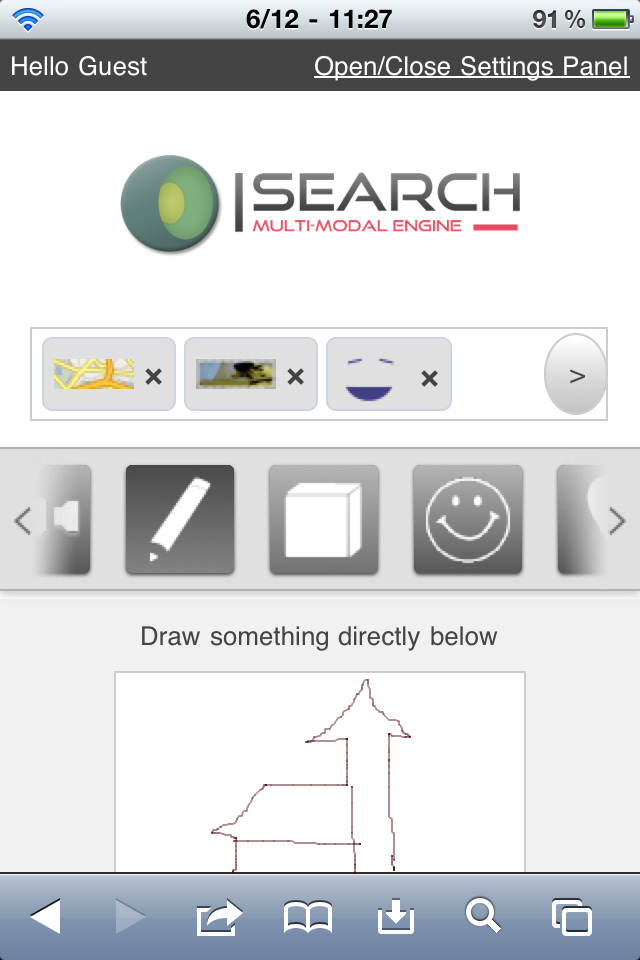
\includegraphics[width=0.72\columnwidth]{./resources/isearch.jpg}
      \label{fig:isearch}}
    \qquad
    \subfloat[][Running on some mobile devices with different screen sizes and operating systems.]{
      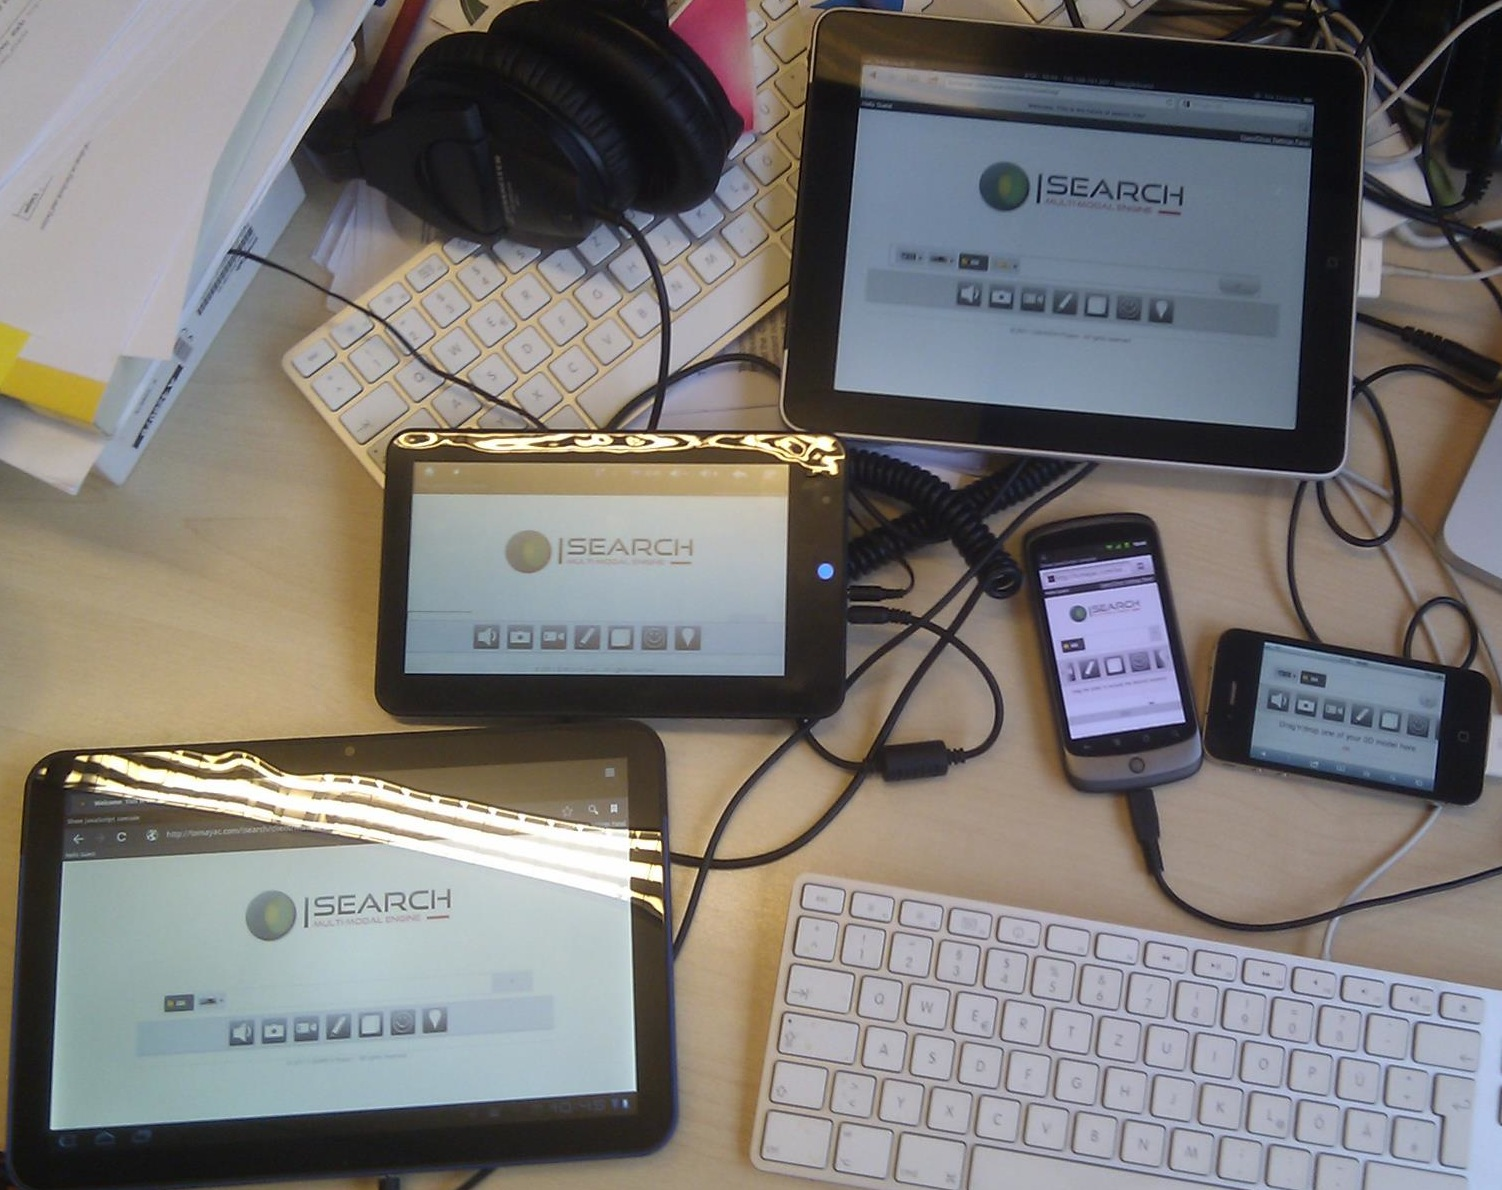
\includegraphics[width=0.72\columnwidth]{./resources/devices.jpg}
      \label{fig:devices}}
    \qquad
    \subfloat[][Treemap results visualization showing different clusters of images.]{
      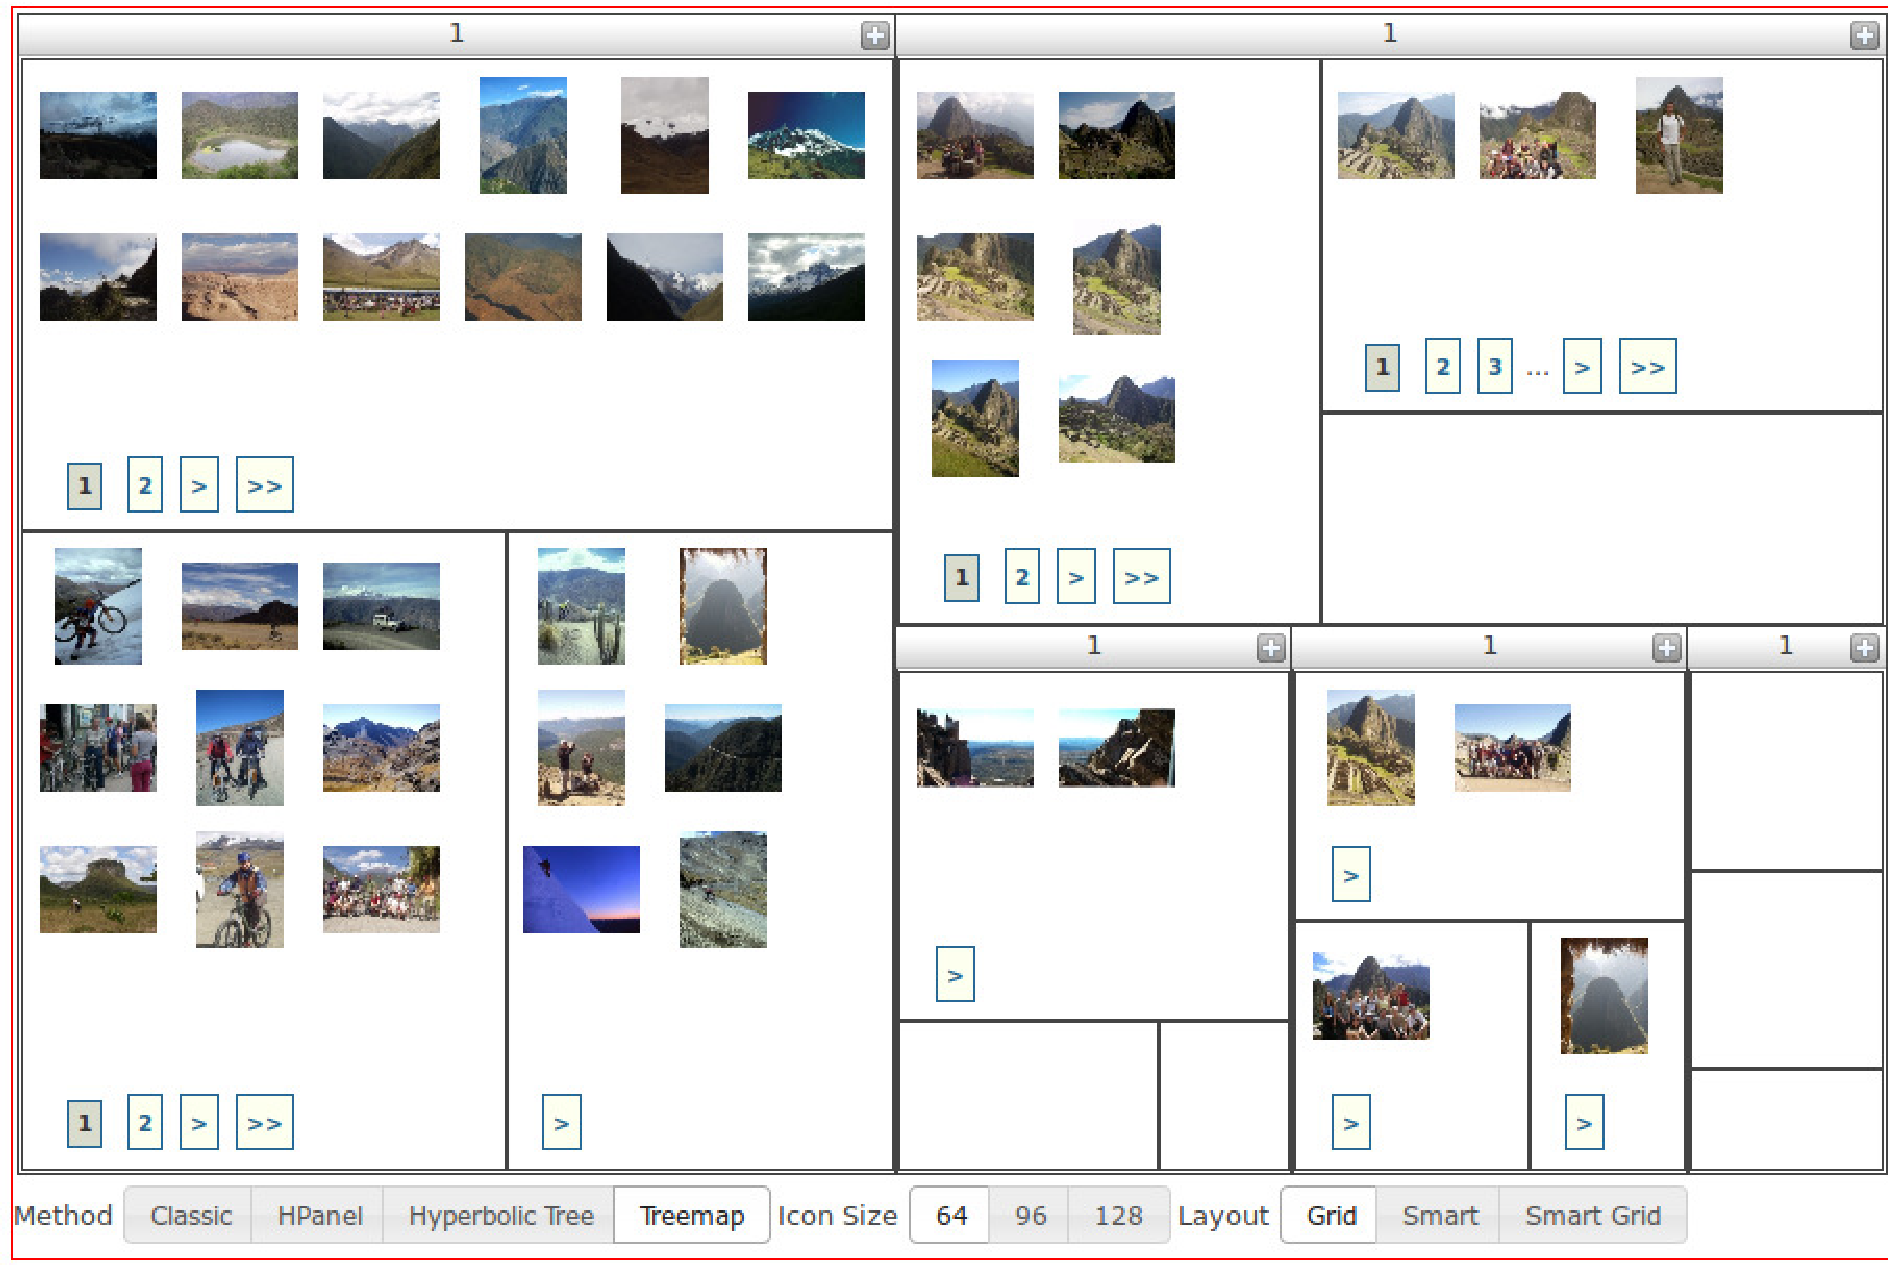
\includegraphics[width=0.72\columnwidth]{./resources/treemap.pdf}
      \label{fig:treemap}}      
\caption{\mbox{I-SEARCH} graphical user interface.}
\label{fig:gui}
\end{figure}

\subsection{Video and Image}
The video mining component produces a video summary as a set of recurrent image patches to give a visual representation of the video to the user.
These patches can be used to refine search and/or to navigate more easily in videos or images.
For this purpose, we use a technique of Letessier \textit{et al.}~\cite{Letessier11} consisting of a weighted and adaptive sampling strategy aiming to select the most relevant query regions from a set of images.
The images are the video key frames and a new clustering method is introduced that returns a set of suggested object-based visual queries. The image search component performs approximate vector search on either local or global image descriptors to speed up response time on large scale databases.

\begin{lstlisting}[caption=Sample \emph{RUCoD} snippet (namespace declarations and some details removed for legibility reasons).,label={lst:rucod}]
<RUCoD>
  <Header>
    <ContentObjectType>
      Multimedia Collection
    </ContentObjectType>
    <ContentObjectName xml:lang="en-US">
      AM General Hummer
    </ContentObjectName>
    <ContentObjectID/>
    <ContentObjectVersion>1</ContentObjectVersion>
    <ContentObjectCreationInformation>
      <Creator>
        <Name>CoFetch Script</Name>
      </Creator>
    </ContentObjectCreationInformation>
    <Tags>
      <MetaTag name="UserTag" type="xsd:string">
        Hummer
      </MetaTag>
    </Tags>
    <ContentObjectTypes>
      <MultimediaContent type="Object3d">
        <FreeText>
          This is not Mirza's model.
        </FreeText>
        <MediaName>2001 Hummer H1</MediaName>
        <MetaTag name="UserTag" type="xsd:string">
          Hummer
        </MetaTag>
        <MediaLocator>
          <MediaUri>
            http://sketchup.google.com/[...]
          </MediaUri>
          <MediaPreview>
            http://sketchup.google.com/[...]
          </MediaPreview>
        </MediaLocator>
        <MediaCreationInformation>
          <Author>
            <Name>ZXT</Name>
          </Author>
          <Licensing>
            Google 3D Warehouse License
          </Licensing>
        </MediaCreationInformation>
        <Size>1840928</Size>
      </MultimediaContent>
      <RealWorldInfo>
        <MetadataUri filetype="rwml">
          AM_General_Hummer.rwml
        </MetadataUri>
      </RealWorldInfo>
    </ContentObjectTypes>
  </Header>
</RUCoD>
\end{lstlisting}

\subsection{Audio and Emotions}
\mbox{I-SEARCH} includes the extraction of expressive and emotional information conveyed by a user to build a query, and the possibility to build queries resulting from a social verbal or non-verbal interaction among a group of users.
The I-SEARCH platform includes algorithms for the analysis of non-verbal emotional behavior expressed by full body gestures, for the analysis of the social behavior in a group of users, and  methods to extract real-world data.

\subsection{3D Objects}
The 3D object descriptor extractor is the component for extracting low level features from 3D objects and is invoked during the content analytics process.
More specifically, it takes as input a 3D object and returns a fragment of low level descriptors fully compliant with the \emph{RUCoD} format.

\subsection{Visualization}
\mbox{I-SEARCH} uses sophisticated information visualization techniques that support not only querying information, but also browsing techniques for effectively locating relevant information.
The presentation of search results is guided by analytic processes such as clustering and dimensionality reduction that are performed after the retrieval process and intend to discover relations among the data.
This additional information is subsequently used to present the results to the user by means of modern information visualization techniques such as treemaps, an example of such can be seen in Subfigure \autoref{fig:treemap}.
The visualization interface is able to seamlessly mix results from multiple modalities
 
\subsection{Orchestration}
One project partner is involved in the orchestration of the particular components of the other partners.
In this context, a so-called \emph{Content Analytics Controller (CAC)} has been developed, which is the component in charge of orchestrating the content analytics process for content object enrichment via low level description extraction.
As a second component, a \emph{RUCoD} authoring tool was built.

\subsection{Content Providers}
The first content provider in the \mbox{I-SEARCH} projects holds an important Italian ethnomusicology archive.
The partner makes available all of its digital content to the project as well as its expertise for the development of requirements and use cases related to music.
The second content provider is an office furniture dealer with a big catalogue of individually customizable pieces of furniture. 
Both partners are also actively involved in user testing and the overall content collection effort for the project via deployed Web services that return their results in the \emph{RUCoD} format.

\section{System Demonstration} \label{sec:systemdemonstration}
With \mbox{I-SEARCH} being in its second year, there is now some basic functionality in place.
We maintain a bleeding-edge demonstration server\footnote{Demonstration: \url{http://isearch.ai.fh-erfurt.de/}}, and have recorded a screencast\footnote{Screencast: \url{http://youtu.be/-chzjEDcMXU}} that shows some of the interaction patterns.
The GUI runs on both mobile and desktop devices, and adapts dynamically to the available screen real estate, which, especially on mobile devices, can be a challenge.
Supported input modalities at this point are \emph{audio}, \emph{video}, \emph{rhythm}, \emph{image}, \emph{3D object}, \emph{sketch}, \emph{emotion}, \emph{geolocation}, and \emph{text}.
For \emph{emotion}, an innovative emotion slider open source solution~\cite{emotionslider} was adapted to our needs.
The GUI supports \textit{drag and drop} user interactions and we aim for supporting low level device access for audio and video uploads.
For \emph{3D objects}, we support Web GL powered 3D views of models.
\emph{Text} can be entered via speech input based on the WAMI toolkit~\cite{wami}, or via keyboard.
First results can be seen upon submitting a query, and the visualization component allows to switch back and forth between different views.

\section{Related Work} \label{sec:relatedwork}
We start covering related work with a differentiation of terms.
\emph{Multimodal search} can be used in two senses; (i), in the sense of multimodal result output based on unimodal query input, and (ii), in the sense of both multimodal result output and multimodal query input.
We follow the second definition, i.e., require the query input interface to allow for multimodality.
We do not consider the first definition, as common search engines already by default return multimodal results.

An interesting multimodal search engine was developed in the scope of the PHAROS project~\cite{pharos2009}.
While the initial query is still keyword-based, the search engine allows for refinements in form of facets, like location, that can be considered modalities.
\mbox{I-SEARCH} develops this concept one step further by supporting multimodality from the beginning.
In~\cite{multimodalitysun}, Rahn Frederick discusses the importance of multimodality in search-driven on-device portals, i.e., handset-resident mobile applications, often preloaded, that enhance the discovery and consumption of endorsed mobile content, services, and applications.
Consumers can navigate on-device portals by searching with text, voice, and camera images.
Rahn Frederick's article is relevant, as it is specifically focused on mobile devices, albeit the scope of \mbox{I-SEARCH} is broader in the sense of also covering desktop devices. 
In a W3C Note~\cite{w3cmultimodal2003}, Larson \textit{et al.} describe a multimodal interaction framework, and identify the major components for multimodal systems.
The multimodal interaction framework is not an architecture \textit{per se}, but rather a level of abstraction above an architecture and identifies the markup languages used to describe information required by components and for data flows among components.
With Mudra~\cite{mudra2011}, Hoste \textit{et al.} present a unified multimodal interaction framework supporting the integrated processing of low level data streams as well as high level semantic inferences.
Their architecture is designed to support a growing set of input modalities as well as to enable the integration of existing or novel multimodal fusion engines.
Input fusion engines combine and interpret data from multiple input modalities in a parallel or sequential way.
\mbox{I-SEARCH} is a search engine that captures modalities sequentially, however, processes them in parallel.

\section{Future Work and Conclusion} \label{sec:futureworkconclusion}
The efforts in the coming months will focus on integrating the different components.
Interesting challenges lie ahead with the presentation of results and result refinements.
In order to test the search engine, a set of use cases has been compiled that covers a broad range of modalities, and combinations of such.
We will evaluate those use cases and test the results in user studies involving customers of the industry partners in the project.

In this paper, we have introduced and motivated the \mbox{I-SEARCH} project and have shown the involved components from the different project partners.
We have then presented first results, provided a system demonstration, and positioned our project in relation to related work in the field.
\mbox{I-SEARCH} is now in a decisive phase of the project, where the components function in isolation, however, need to be integrated in order to work well in orchestration with the entire \mbox{I-SEARCH} framework.
The coming months will be fully dedicated to the integration efforts and we are optimistic to successfully evaluate the set of use cases in the project's final year.

\section{Acknowledgments}
This work was partially supported by the European Commission under Grant No. 248296 FP7 \mbox{I-SEARCH} project.

% back to normal size Computer Modern for URLs in bibliography
\let\ttdefault\oldttdefault
\let\url\oldurl

\bibliographystyle{abbrv}
\bibliography{www2012}

\balancecolumns
\end{document}